\section{Exploring the Data}
\label{sec:Exploring the Data}

\subsection{Relationships Dataset}
\label{subsec:Relationships Dataset}

\begin{figure}[H]
\begin{center}
    \begin{subfigure}[b]{0.45\textwidth}
        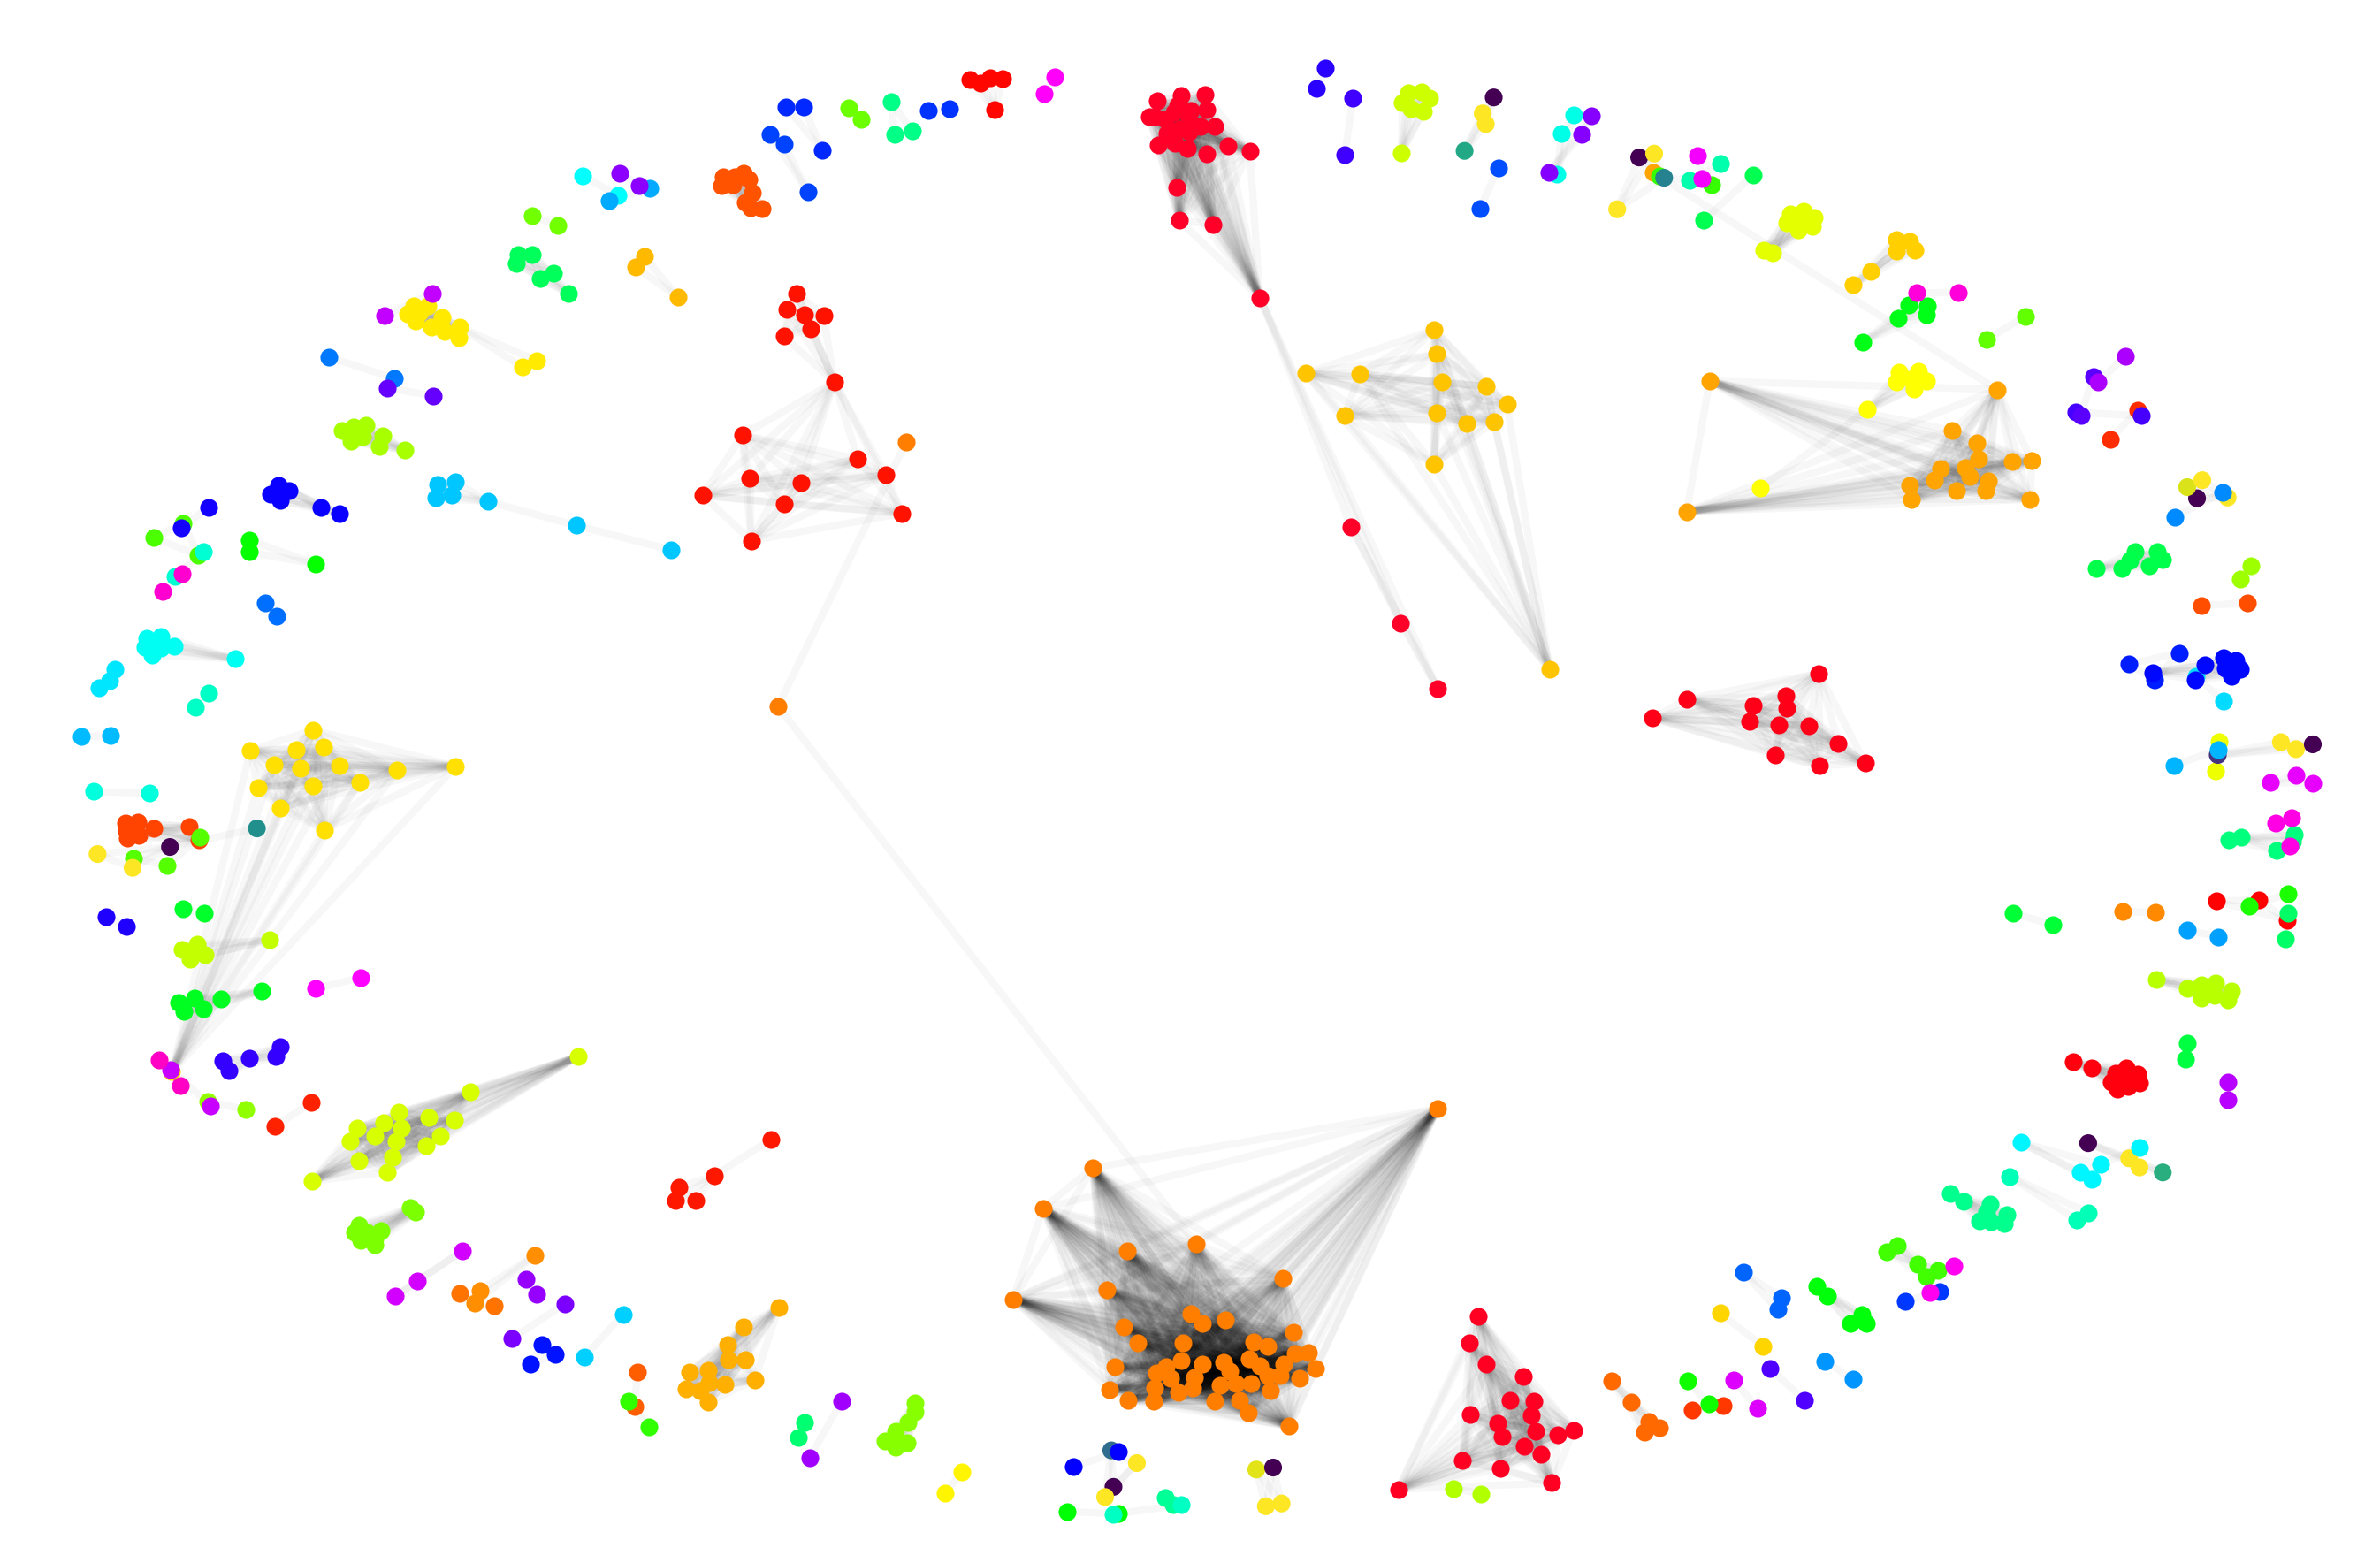
\includegraphics[width=\textwidth]{graphLoc.png}
        \caption{Terror attacks location graph, colouring by component ID}
        \label{fig:graphLoc}
    \end{subfigure}
    ~
    \begin{subfigure}[b]{0.45\textwidth}
        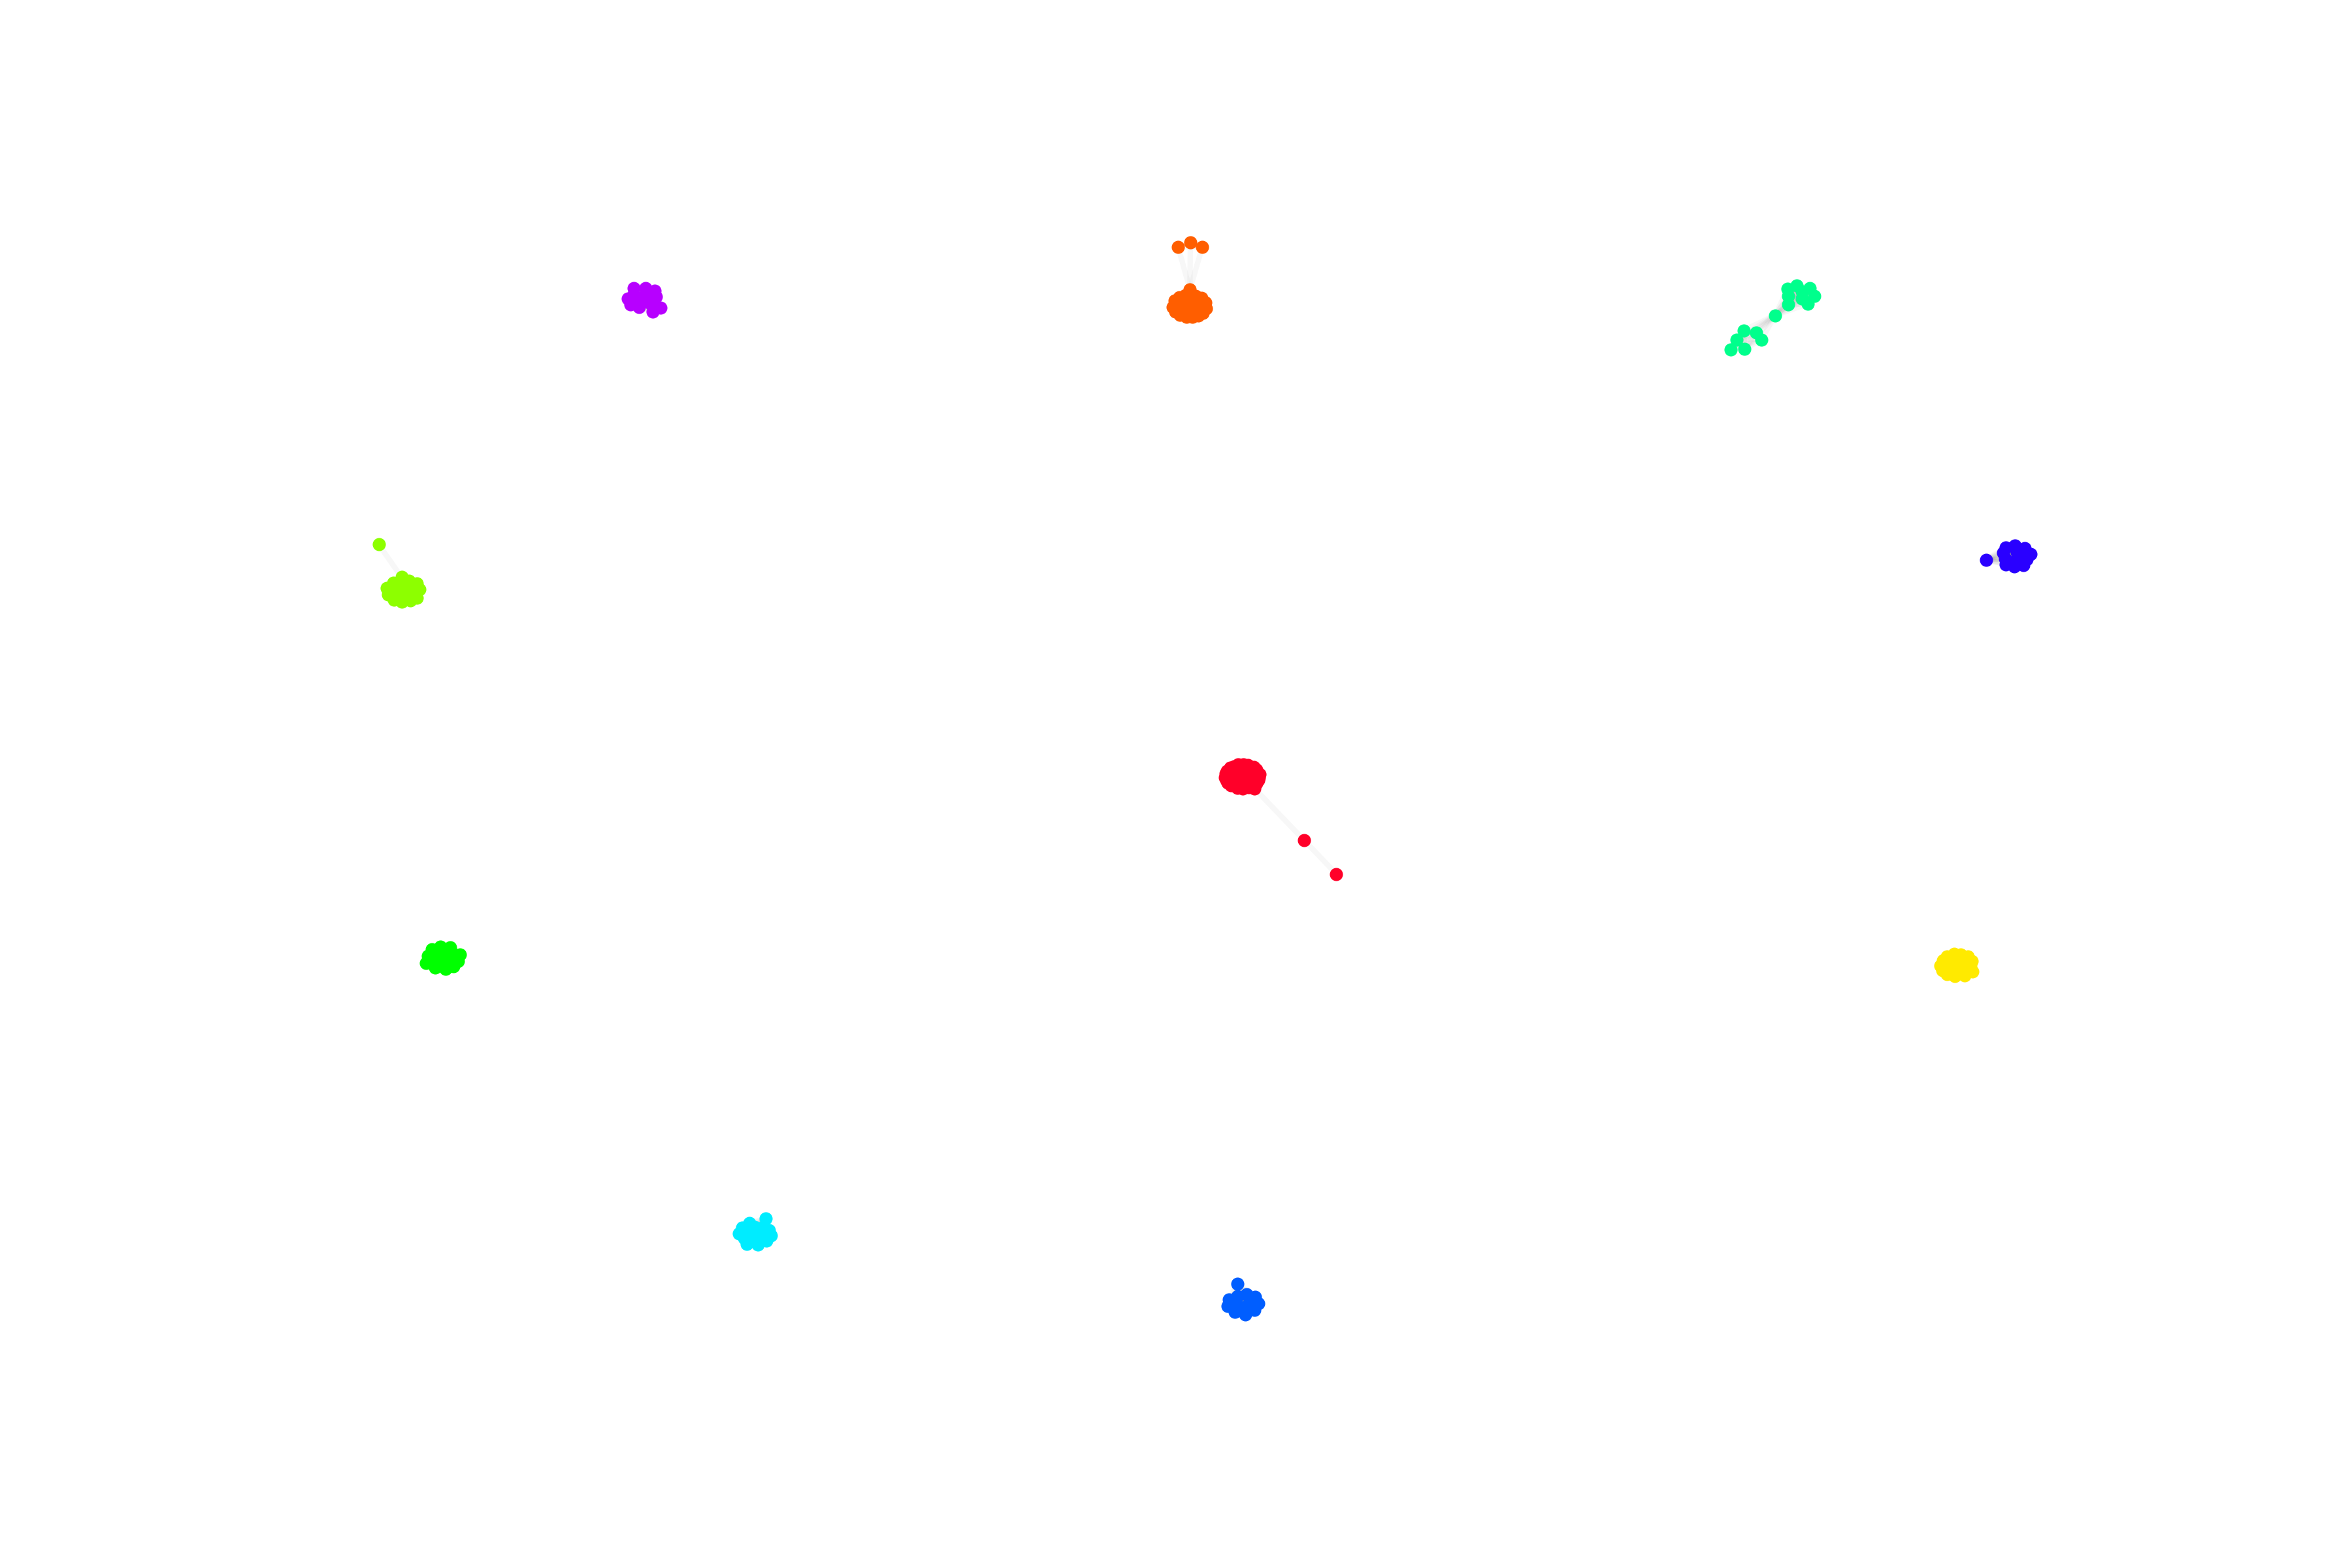
\includegraphics[width=\textwidth]{subGraph.png}
        \caption{Ten biggest components from the terror attacks location graph}
        \label{fig:subGraph}
    \end{subfigure}
\caption{Graphs analysed in the project}
\label{fig:graphPlots}
\end{center}
\end{figure}

\subsection{Terror Attacks Dataset}
\label{subsec:Terror Attacks Dataset}

The formation of the network implies a transitive relation between most of the nodes. Indeed, if for most nodes, take $a$ $b$ and $c$ in the network, we have
\begin{equation}
a \sim b \text{ and } b \sim c \text{ then } a \sim c 
\end{equation}
Equivalently, if attack $a$ took place close to $b$, and attack $b$ took place close to $c$, then it is probable that attack $a$ took place close to $c$.